\chapter{Introduction} 

\section{Introduction to Flood Prediction and Early Warning System}

Flooding is one of the most common natural disasters in the world and has consistently posed major threats to human lives, infrastructure, and national economies. In Thailand, flood events have repeatedly caused widespread damage, particularly in low-lying river basins and densely populated provinces. With climate change intensifying rainfall variability and increasing the frequency of extreme weather, the impact of floods has become more challenging to predict and manage. Therefore, early warning systems and predictive models are increasingly essential for mitigating risks and supporting timely decision-making.

Flood prediction and early warning systems aim to provide actionable forecasts based on hydrological and meteorological conditions, enabling communities and responsible agencies to prepare for possible flood events. Traditional forecasting systems often rely heavily on physical hydrological models or manual monitoring and may not provide localized or timely predictions in all regions. With improvements in data availability and computational power, machine learning has emerged as a viable alternative, allowing systems to learn from historical patterns and make short-term water level predictions with improved responsiveness. However, effective data handling and proper predictive modeling are required.

\begin{figure}[htbp]
    \centering
    % Ensure your file path is correct
    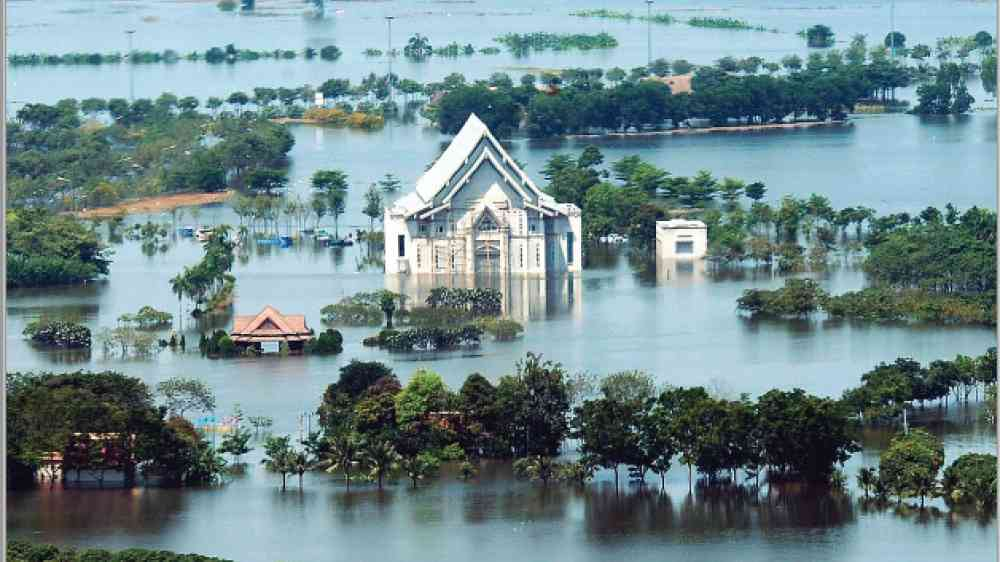
\includegraphics[width=0.95\textwidth]{figures/figure1.jpg}
    \caption{2011 Thailand's Flood.}
    \label{fig:complete_grid}
\end{figure}

\section{Global perspective of Flood}

According to the World Meteorological Organization (WMO, 2025)\cite{wmo2025floods}, floods account for nearly 40 percent of all natural disasters worldwide and have been the most widespread natural hazard globally. From flash floods in rural areas to large-scale river floods, no region remains unaffected. The number of flood-related events has increased significantly over the past decades, driven largely by rising global temperatures and erratic rainfall patterns. Moreover, rapid urbanization and land-use changes have further worsened flood risks by reducing natural drainage and increasing surface runoff. These conditions emphasize the urgent need for robust flood forecasting solutions and scalable early warning mechanisms, especially as climate change continues to deviate global weather patterns.

\section{Local Perspective of Flood (Thailand)}

Since Thailand is also regarded as one of the most vulnerable countries to climate-related disasters in Southeast Asia, floods remain one of the most frequent and devastating threats to humans. As stated by (Nation, 2024)\cite{thenation2024ongoing}, nearly 26,000 households in both the Northern and Eastern regions of Thailand are still overwhelmed by flooding, and 46 people have drowned to death, while 24 have sustained injuries as of the date 16th August 2025.

\begin{figure}[htbp]
    \centering
    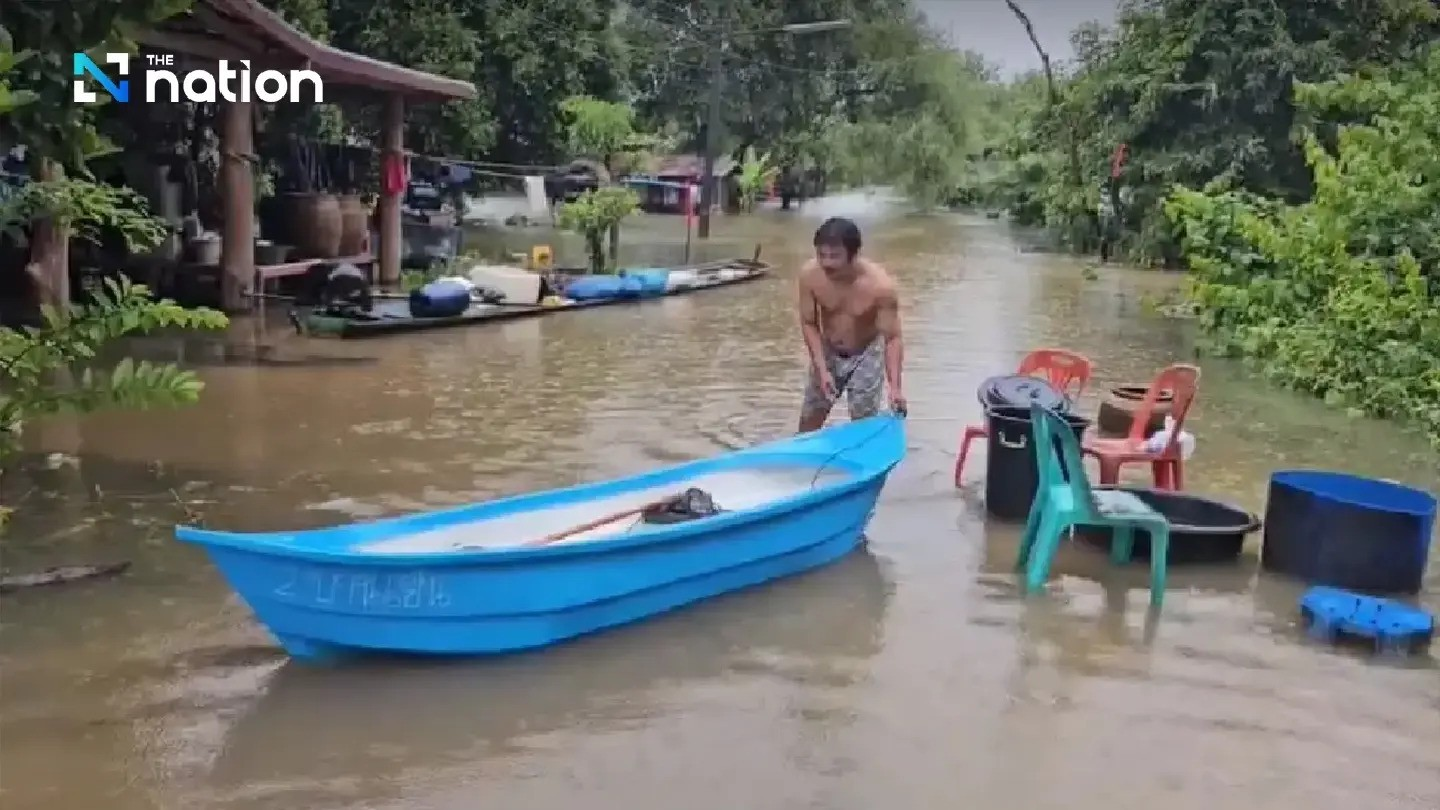
\includegraphics[width=\linewidth]{figures/figure2.jpg}
    \caption{Impact of Thailand’s flood in 2025.}
    \label{fig:impact_thailand_flood}
\end{figure}

\section{Why Do We Do This Project?}

\begin{table}[htbp]
    \centering
    \caption{Project Motivation and Rationale}
    \label{tab:motivation}
    \begin{tabular}{l p{10cm}}
        \hline
        \textbf{Motivation} & \textbf{Description} \\
        \hline
        \textbf{Public Safety} & Early flood warnings save lives and protect property. \\
        \textbf{Critical Location} & Krungthep Bridge is a key monitoring point in Bangkok. \\
        \textbf{Data Availability} & 6+ years of hourly water level data (2019-2025). \\
        \textbf{Technical Challenge} & Complex temporal patterns require advanced ML approaches. \\
        \textbf{Real-world Application} & Results can be deployed for actual flood monitoring. \\
        \hline
    \end{tabular}
\end{table}

\section{Problem Statement}

The problem we aim to solve is: ``How can we build a predictive system that accurately forecasts water levels and provides early warnings to reduce the losses caused by floods in Thailand?''

The proposed solution is a data-driven flood prediction and early warning system using supervised machine learning to forecast in the following manner.

\vspace{0.5em}
\noindent \textbf{Inputs:}
\begin{itemize}
    \item Water level (hourly)
    \item Meteorological data (temperature, wind, humidity, pressure, rainfall)
    \item River discharge
    \item Temporal features (hour, month, cyclical encoding)
\end{itemize}

\noindent \textbf{Outputs:}
\begin{itemize}
    \item 24-hour future water-level forecasts (continuous)
    \item Risk levels (categorical) based on bank capacity thresholds
    \item Used for Thailand’s river monitoring and forecasting
    \item Uses real-time weather data from Open-Meteo
\end{itemize}

\subsection{Possible Users}
\begin{enumerate}
    \item \textbf{Various agencies:} Infrastructure managers, including municipalities, as well as the Hydro-informatics Institute (HII).
    \item \textbf{Emergency responders:} Need precise flood forecasts to facilitate evacuation plans.
    \item \textbf{Farmers and communities who live in flood-prone areas:} Rely on early warnings to safeguard crops, livestock, and property.
\end{enumerate}